\documentclass{beamer}
%%%%%%%%%%%%%%%%%%%%%%%%%%%%%%%  Packages  %%%%%%%%%%%%%
\usepackage{amsmath} 
\usepackage{mathtools}
\usepackage{physics}
\usepackage{amssymb}
\usepackage{mathptmx}
\usepackage{array}
  
%%%%%%%%% FIGurES %%%%%%%%%%%%%%%%%%%%%%%%
\usepackage{textcomp}
\usepackage{graphicx}
\usepackage{caption} 
\usepackage{subcaption}
\usepackage{scrextend}
\usepackage{rotating}
\usepackage{float}
\usepackage{hyperref}

\graphicspath{{./figures/}}
\hypersetup{colorlinks=true, citecolor=blue, linkcolor=blue}
\renewcommand{\equationautorefname}{Eq.}
\renewcommand{\figureautorefname}{Fig.}
 
%%%%%%%%%%%% LaNgUaGe %%%%%%%%%%%%%%%%%%
\usepackage{verbatim}
\usepackage{natbib}
%\usepackage{qcircuit}
\usepackage{wrapfig}

\usepackage{minted}

\usepackage[utf8]{inputenc}
\usetheme{PaloAlto}

\setminted[bash]{breaklines}

\title{Version control using Git and Plotting Tutorial}
\author{Oliver Thomas}
\institute{Quantum Engineering CDT \\ University of Bristol}
\date{\today}

% plan


\begin{document}

\frame{\titlepage}



\begin{frame}{Overview}


\begin{itemize}
        \item Version control using Git
        \item Plotting using Gnuplot
        \item Text editing using Vim
    \end{itemize}
\end{frame}

% slide 1
\begin{frame}
\frametitle{Why you should use version control}
\begin{itemize}
	\item Does this seem familiar? 
\end{itemize}

\begin{figure}[H]
	\centering
	
\includegraphics[width=0.26\textwidth]{xkcdversion.png}
	\caption{Bad version control\footnote{\url{https://xkcd.com/1459/}}}
	\label{fig:xkcdversion}
\end{figure}
\end{frame}

%slide 2
\begin{frame}
\frametitle{What is Git?}
\begin{itemize}
\item Git is one of most used version control software in the world 
\item Git is cross-platform and easy to use \footnote{\url{https://try.github.io/levels/1/challenges/1}}
\end{itemize}
\end{frame}

%slide 2
\begin{frame}
\frametitle{What is GitHub?}
\begin{itemize} 
\item Github is a cloud service for git which lets you store your repository online
\item Why would you store your repository online?
\begin{itemize}
\item Working remotely
\item Collaborative work  
\item Hard drive failure!
\end{itemize}
\end{itemize}
\end{frame}


%slide 3
\begin{frame}
\frametitle{Making a repository}
\begin{itemize}
\item You can do this online on the Github website \footnote{\url{https://github.com/}}
\item Create a new repository
\item Then click clone to get the url, open git on your computer and type: \\ 
	\texttt{git clone url}
\end{itemize}
\end{frame}

%slide 3
\begin{frame}
\frametitle{Making a repository}
\begin{itemize}
	\item Go to the folder and right click \texttt{git with bash}
\item You are now able to use bash for the rest of the talk!
\end{itemize}
\end{frame}

%slide 4
\begin{frame}
\frametitle{Basic Git commands}
\begin{itemize}
	\item There are four\footnote{I cheat here and write a bash script which does these in order so I only have to run a single command.} important commands you will need for git:
	\item \texttt{git pull}
	\item \texttt{git add *}
	\item \texttt{git commit -a}
	\item \texttt{git push}
\end{itemize}
\end{frame}

%slide 2
\begin{frame}
	\frametitle{Adding your first commit}
    Every repository should contain a readme, make one now then run:
\begin{itemize}
	\item \texttt{git add *}
	\item \texttt{git commit -a}
	\item \texttt{git push}
\end{itemize}

Or use the windows GUI version and commit them to your repository.
\end{frame}

%%%%%%%%%%%%%%%%%%%%%%%%%%%%%%%%%%%%%%%%%%%%%%%%%%%%%%%%%%%%%%%%%%%%%%%%%%%%%
%slide 2
\begin{frame}
\frametitle{Branching}
\begin{itemize}
\item Branching is useful, it lets you test something out separately to the main branch.
\item To make a new branch called \texttt{test} \\
\texttt{git branch test} 
\item You can check all of the current branches and which branch you are on with \\
	\texttt{git branch}
\end{itemize}
\end{frame}

%slide 2
\begin{frame}
\frametitle{Branching}
\begin{itemize}
	\item To switch to the test branch type: \\ 
	\texttt{git checkout test} \\
\end{itemize}
\end{frame}

%slide 4
\begin{frame}
\frametitle{Adding Collaborators}
\begin{itemize}
	\item Go to a repository and on the settings tab click collaborators, you can then search using a github username
\end{itemize}
\end{frame}

%slide 4
\begin{frame}
\frametitle{Advanced Git commands}
\begin{itemize}
    \item One of the great things about Git is that you can get by with just the four (main) commands mentioned earlier.
	\item The git man page is very useful, especially, \\
	\texttt{man gittutorial} \\
	\texttt{man giteveryday} \\ 
\item \texttt{giteveryday} is a super useful collection of the 20 commands you will need regularly.
\end{itemize}
\end{frame}

%%%%%%%%%%%%%%%%%%%%%%%%%%%%%%%%%%%%%%%%%%%%%%%%%%%%%%%%%%%%%%%%
%slide 5
\begin{frame}
\frametitle{Gnuplot} 
\begin{itemize}
	\item Gnuplot is popular, multi-platform and standard software on computing clusters\footnote{standard on most of the popular linux distributions} 
    \item \url{https://sourceforge.net/projects/gnuplot/files/gnuplot/5.2.4}
\end{itemize}
\end{frame}

%%%%%%%%%%%%%%%%%%%%%%%%%%%%%%%%%%%%%%%%%%%%%%%%%%%%%%%%%%%%%%%%%
%slide gnuplot 1
\begin{frame}[fragile]
    \frametitle{Example 0 Quick plotting}
\begin{itemize}
	\item Go to the \texttt{src} folder
    \item open gnuplot and type \\ \texttt{plot 'data.txt'}
\end{itemize}
\end{frame}

%slide 2
\begin{frame}{Example 0 Quick plotting}
    \begin{figure}
	\centering
	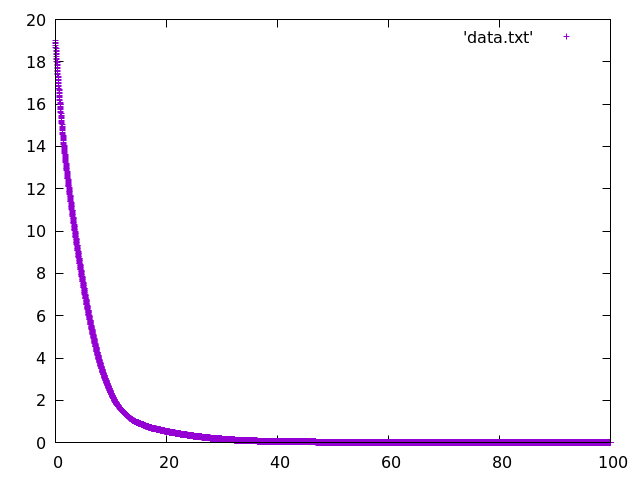
\includegraphics[width=0.6\textwidth]{src/data.png}
	\caption{function plotting}
	\label{fig:function}
\end{figure}
Lets you very quickly see what the data is doing
\end{frame}

%%%%%%%%%%%%%%%%%%%%%%%%%%%%%%%%%%%%%%%%%%%%%%%%%%%%%%%%%%%%%%
%slide gnuplot 1
\begin{frame}[fragile]
    \frametitle{Example 1 Plotting functions}
\begin{itemize}
	\item Go to the \texttt{src} folder
    \item open gnuplot and type \\ \texttt{load 'ex1\_basic.p'}
\end{itemize}
\inputminted[fontsize=\small]{bash}{src/ex1_basic.p}
\end{frame}

%slide saving plots gnuplot 
\begin{frame}[fragile]
    \frametitle{Example 2 Saving plots}
\begin{itemize}
	\item Go to the \texttt{src} folder
    \item open gnuplot and type \\ \texttt{load 'ex2\_saving.p'}
\end{itemize}
\inputminted[fontsize=\small]{bash}{src/ex2_saving.p}
\end{frame}

%slide 2
\begin{frame}{Example 2 Plotting functions}
    \begin{figure}
	\centering
	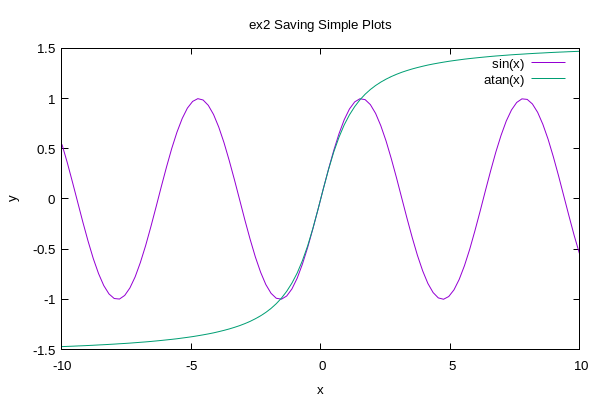
\includegraphics[width=0.6\textwidth]{src/ex2.png}
	\caption{function plotting}
	\label{fig:function}
\end{figure}
Produces a png
\end{frame}

%%%%%%%%%%%%%%%%%%%%%%%%%%%%%%%%%%%%%%%%%%%%%%%%%%%%%%%%%%%%%%%%
%slide 2
\begin{frame}[fragile]
\frametitle{Example 3 Plotting data}
\begin{itemize}
	\item open gnuplot and type \\ \texttt{load 'ex3\_barchart.p}
\end{itemize}
\inputminted[fontsize=\small, firstline=8]{bash}{src/ex3_barchart.p}
\end{frame}

%slide 2
\begin{frame}
\frametitle{Example 3 Plotting data}
\begin{figure}
	\centering
	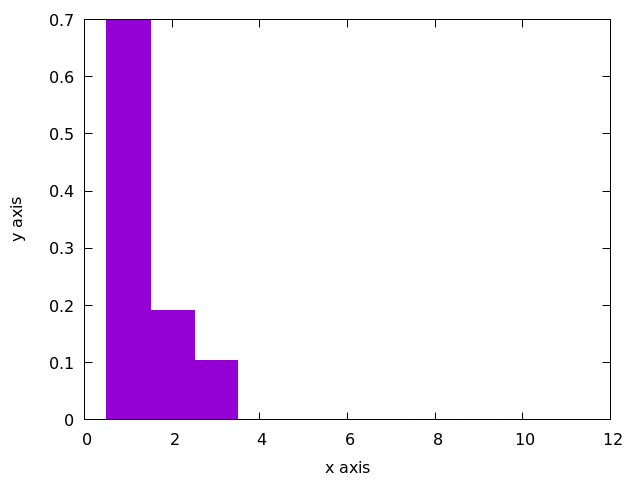
\includegraphics[width=0.5\textwidth]{src/ex3.png}
	\caption{function plotting}
	\label{fig:function}
\end{figure}
\end{frame}



%%%%%%%%%%%%%%%%%%%%%%%%%%%%%%%%%%%%%%%%%%%%%%%%%%%%%%%%%%%%%%%%
%slide subplots
\begin{frame}[fragile]
\frametitle{Example 4 Subplots}
\begin{itemize}
\item open gnuplot \\ \texttt{load 'ex4\_multiplot.p'} 
\end{itemize}
\inputminted[fontsize=\small, firstline=4, lastline=9]{bash}{src/ex4_multiplot.p}
\inputminted[fontsize=\small, firstline=14, lastline=15]{bash}{src/ex4_multiplot.p}
\inputminted[fontsize=\small, firstline=27, lastline=28]{bash}{src/ex4_multiplot.p}
\end{frame}

%slide 2
\begin{frame}
\frametitle{Example 4 Subplots}
\begin{figure}
	\centering
	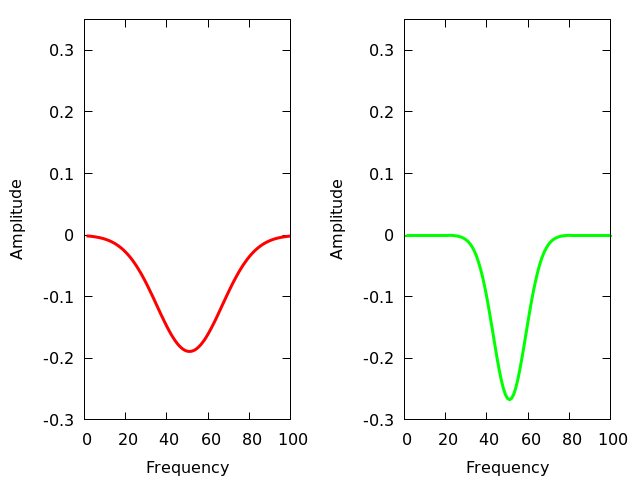
\includegraphics[width=0.5\textwidth]{src/ex4.png}
	\caption{function plotting}
	\label{fig:function}
\end{figure}
\end{frame}


%%%%%%%%%%%%%%%%%%%%%%%%%%%%%%%%%%%%%%%%%%%%%%%%%%%%%%%%%%%%%%%%
%slide 2
\begin{frame}[fragile]
\frametitle{Example 5 Surface plots}
\begin{itemize}
\item open gnuplot \\ \texttt{load 'ex5\_splot.p}
\end{itemize}
\inputminted[fontsize=\small]{bash}{src/ex5_splot.p}
\end{frame}

%slide 2
\begin{frame}
\frametitle{Example 5 Surface plots}
\begin{figure}
	\centering
	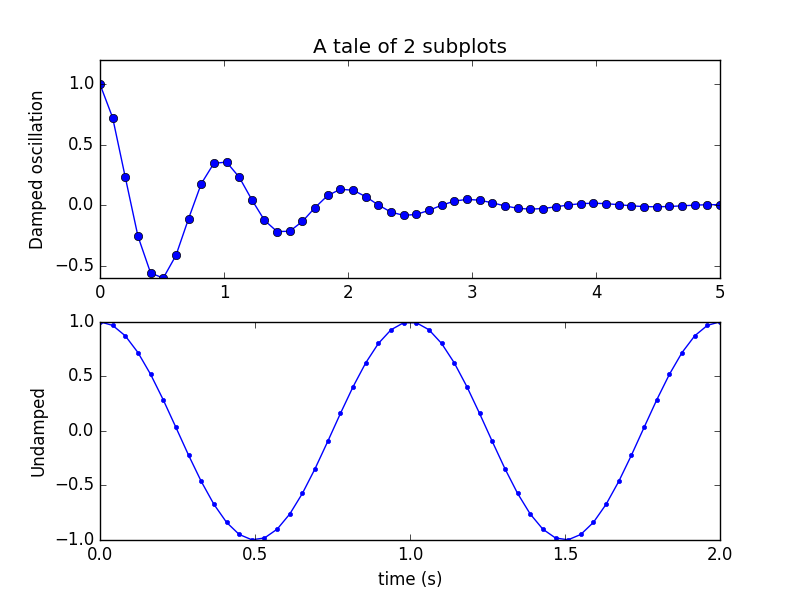
\includegraphics[width=0.6\textwidth]{src/ex5.png}
	\caption{function plotting}
	\label{fig:function}
\end{figure}
\end{frame}

%%%%%%%%%%%%%%%%%%%%%%%%%%%%%%%%%%%%%%%%%%%%%%%%%%%%%%%%%%%%%%%
\begin{frame}
    \frametitle{Gnuplot summary \& features}
    \begin{itemize}
        \item The documentation is very good, there will be an example of whatever you want to do somewhere
        \item You can set \textit{pointstyle}, \textit{linestyle}, and colours 
        \item Very easy to generate quick plots
        \item Scripts makes it easy to generate nice figures
        \item You can make GIFs
    \end{itemize}
\end{frame}

%%%%%%%%%%%%%%%%%%%%%%%%%%%%%%%%%%%%%%%%%%%%%%%%%%%%%%%%%%%%%%%%

% slide editors
\begin{frame}{A brief note on text editors: Vim}
    \begin{itemize}
    \item Vim is a powerful cross-platform text editor, released in 1991 and is still regarded as one of the most popular editors \footnote{Along with Emacs}. 
    \item Flexible with thousands of plugins available e.g. I use Vim to compile latex documents, this presentation was written in Vim.  
    \item Computing clusters normally only have CLI so if you are running high performance code you will need to be familiar with Vim, Emacs or Nano.
    \item Overleaf supports Vim keybindings
    \item You can feel like a Hacker.
\end{itemize}
\end{frame}

\begin{frame}{Vim commands}
    \begin{itemize}
        \item The most important thing to remember is that Vim has two main modes, \textit{NORMAL}, \texttt{ESC} and \textit{INSERT}, \texttt{i}
        \item All commands are run from \textit{NORMAL} mode using \texttt{:}
        \item to quit use, \texttt{ESC:q} (meaning go to \textit{NORMAL} mode, \texttt{:} means command and \texttt{q} is quit without saving)
        \item to save and quit use, \texttt{ESC:wq} (\texttt{w} stands for write)
    \end{itemize}
    In case everything goes wrong, \texttt{:q!} is force-quit without saving
\end{frame}

%%%%%%%%%%%%%%%%%%%%%%%%%%%%%%%%%%%%%%%%%%%%%%%%%%%%%%%%%%%%%%%%%%%%%%%%%%%%%%5
\begin{frame}
    \frametitle{Vim commands continued}
    All of these commands are case-sensitive and must be run in \textit{NORMAL} mode not \textit{INSERT} 

    \texttt{v} puts you in visual mode, useful for highlighting a block of text to copy or cut and paste
    \begin{itemize}
        \item \texttt{y} -yank (copy), \texttt{yy} -yank (copy) whole line
        \item \texttt{d} -delete (cut), \texttt{dd} -delete (cut) whole line
        \item \texttt{p} -paste after cursor, \texttt{P} -paste before cursor
    \end{itemize}

    \begin{itemize}

        \item \texttt{x} -delete character
        \item \texttt{u} -undo
        \item \texttt{CTRL R} -redo
    \end{itemize}
\end{frame} 

\begin{frame}
    \frametitle{Movement commands}
    \begin{itemize}
    \item \texttt{a} -append at the end of the next word, \texttt{A} -append at the end of the line
    \item \texttt{o} -open line bellow in \textit{INSERT} mode, \texttt{O} -opens line above in \textit{INSERT} mode
    \item \texttt{0} -go to start of line
    \item \texttt{\$} -go to end of line
    \item \texttt{\{} -go to previous paragraph
    \item \texttt{\}} -go to next paragraph 
    \end{itemize}
\end{frame}

%%%%%%%%%%%%%%%%%%%%%%%%%%%%%%%%%%%%%%%%%%%%%%%%%%%%%%%%%%%%%%%%%%%%%%%%%%%%%
\begin{frame}
    \frametitle{Searching and editing in Vim}
    Searching
    \begin{itemize}
    \item \texttt{fx} -find next occurrence of x in text,\\ e.g. \texttt{f}\textit{b} finds the next letter \textit{b} in a line 
    \item /x -search the whole document for x,\\ e.g. /\textit{b} finds all letter \textit{b}s
\end{itemize}

use \texttt{n} to go to next occurrence, \texttt{N} to go to previous.

Editing
\begin{itemize}
        \item \texttt{r} -replace character, \\ e.g. \texttt{r}\textit{a} replaces character with \textit{a}
        \item \texttt{\~} -Changes the CASE of character, \\ e.g. \texttt{\~} when the cursor is over \textit{a} will change it to a capital, \textit{A} \\ can be used with \textit{VISUAL} mode to block capitalise or block lower-case
    \end{itemize}
        \end{frame}

\begin{frame}
    \frametitle{Using SED in Vim}
     Sed stands for Stream EDitor and can be used directly from vim \footnote{\url{http://vim.wikia.com/wiki/Search_and_replace}} 

     Probably the most regularly used sed commands you will need are,
     \begin{itemize}
    \item :\%s/foo/bar/g -replaces all instances of foo with bar globally
    \item :4,31s/foo/bar/g -replace instances of foo with bar in lines 4-31 
\end{itemize}
\end{frame}

\begin{frame}
    \frametitle{Vim summary}
    \begin{itemize}
    \item You should try Vim, it is available in overleaf
    \item It takes some getting used to, but I and many others think it is worth it.
    \item Cross-platform and powerful
    \item Very good documentation
    \end{itemize}
\end{frame}

%%%%%%%%%%%%%%%%%%%%%%%%%%%%%%%%%%%%%%%%%%%%%%%%%%%%%%%%%%%%%%%%%%%%%%%%%
\begin{frame}
    \frametitle{Conclusion}
    \begin{itemize}
    \item You should use version control
    \item I recomend gnuplot as it is easy to use
    \item Vim is a fantastic editor but does require a small amount of effort to learn
    \end{itemize}
\end{frame}


%slide 2
\begin{frame}
\frametitle{Thanks for listening!}
\begin{figure}[H]
	\centering
	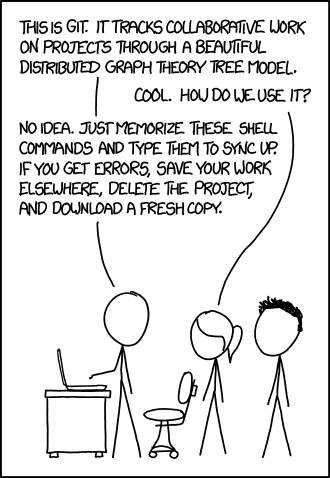
\includegraphics[width=0.4\textwidth]{xkcdgit.png}
	\caption{If it all goes wrong \ldots \footnotemark }
	\label{fig:xkcdversion}
\end{figure}
\footnotetext[1]{\url{https://xkcd.com/1597/}}
\end{frame}


\end{document}
